% From https://www.overleaf.com/learn/latex/Pgfplots_package

\documentclass{report}
\usepackage{tikz}
\usepackage{pgfplots}
\begin{document}
    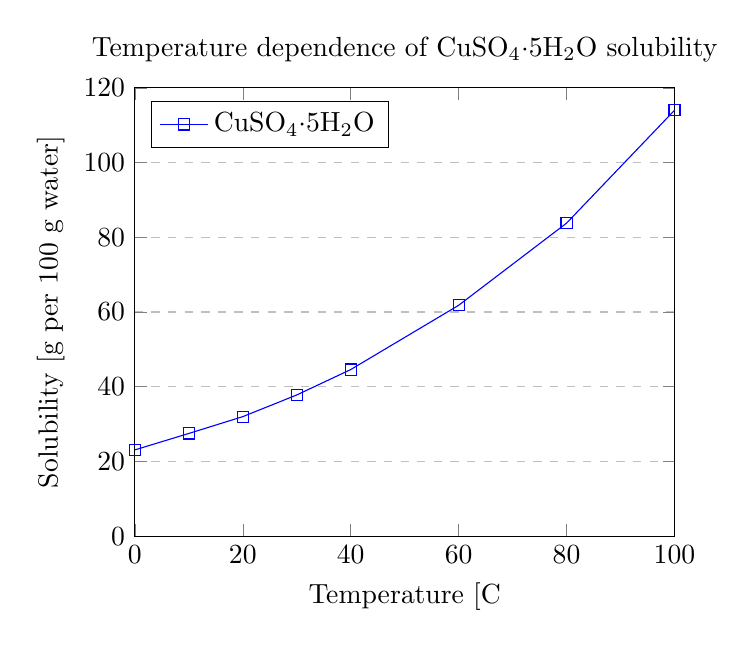
\begin{tikzpicture}
        \begin{axis}[
        title={Temperature dependence of CuSO\(_4\cdot\)5H\(_2\)O solubility},
        xlabel={Temperature [C},
        ylabel={Solubility [g per 100 g water]},
        xmin=0, xmax=100,
        ymin=0, ymax=120,
        xtick={0,20,40,60,80,100},
        ytick={0,20,40,60,80,100,120},
        legend pos=north west,
        ymajorgrids=true,
        grid style=dashed,
        ]

        \addplot[
            color=blue,
            mark=square,
        ]
        coordinates {
            (0,23.1)(10,27.5)(20,32)(30,37.8)(40,44.6)(60,61.8)(80,83.8)(100,114)
        };
        \legend{CuSO\(_4\cdot\)5H\(_2\)O}

        \end{axis}
    \end{tikzpicture}
\end{document}
